\chapter{近简并能带电子的磁性质}

在磁场中布洛赫电子的准经典理论中,量子化条件不仅仅是朗道能级的简洁描述,而且是输运性质\cite{SdH}和热力学性质\cite{dHvA}的量子振荡的定量理论的基石。 Onsager\cite{Onsager}和Lifshitz\cite{lifshitz_kosevich,lifshitz_kosevich_jetp}给出的最初的量子化条件忽略了自旋轨道耦合。随后Roth\cite{rotheffham,rothmag},Mikitik\cite{Mikitik_quantizationrule}以及本文作者及合作者\cite{topoferm,100p}将自旋轨道耦合效应考虑了进来,但是得到的量子化条件仅仅适用于自旋轨道耦合效应远远大于(或者远远小于)塞曼作用能。


到目前为止,我们还没有看到一个能够将自旋轨道耦合和塞曼劈裂同等处理的量子化条件。对于没有空间反演的具有自旋轨道耦合的材料,或者是具有磁序的材料,这样的一个量子化条件非常重要。这些材料具有一个自旋二分之一的自由度,并且能带的自旋简并被自旋轨道耦合或者磁序微弱地劈开。一个典型的例子就是具有Rashba自旋轨道耦合的二维电子气:
\begin{equation}
H_R=\frac{{\hbar^2} k^2}{2m}+\hbar\alpha  (k_{x}\sigma_{y}-k_{y}\sigma_{x}).\label{eq:Rashba-Hamiltonian}
\end{equation}
考虑加上一个$-z$方向的磁场,我们主要关注能量远大于$m\alpha^2$的地方。这里,磁振子轨道【见图\fig{fig:orbits}(a)】在$\bk$空间被自旋轨道耦合劈开,其面积之差为$\delta S$,其中$\delta S$远小于两个轨道的面积的平均值$S$\footnote{式\ref{deltaSvsS}中 $\delta S$ 和 $S$ 的表达式在$E{\gg}m\alpha^2$时渐进正确。}:
\e{\delta S = 4\pi m \alpha k_E/\hbar\ll S =\pi k_E^2; \;\; k_{E}:=\f{\sqrt{2m E}}{\hbar}.\label{deltaSvsS}}
$S$ 也是在没有自旋轨道耦合的时候的磁振子的面积($\alpha{=}0$)。

\begin{figure}
	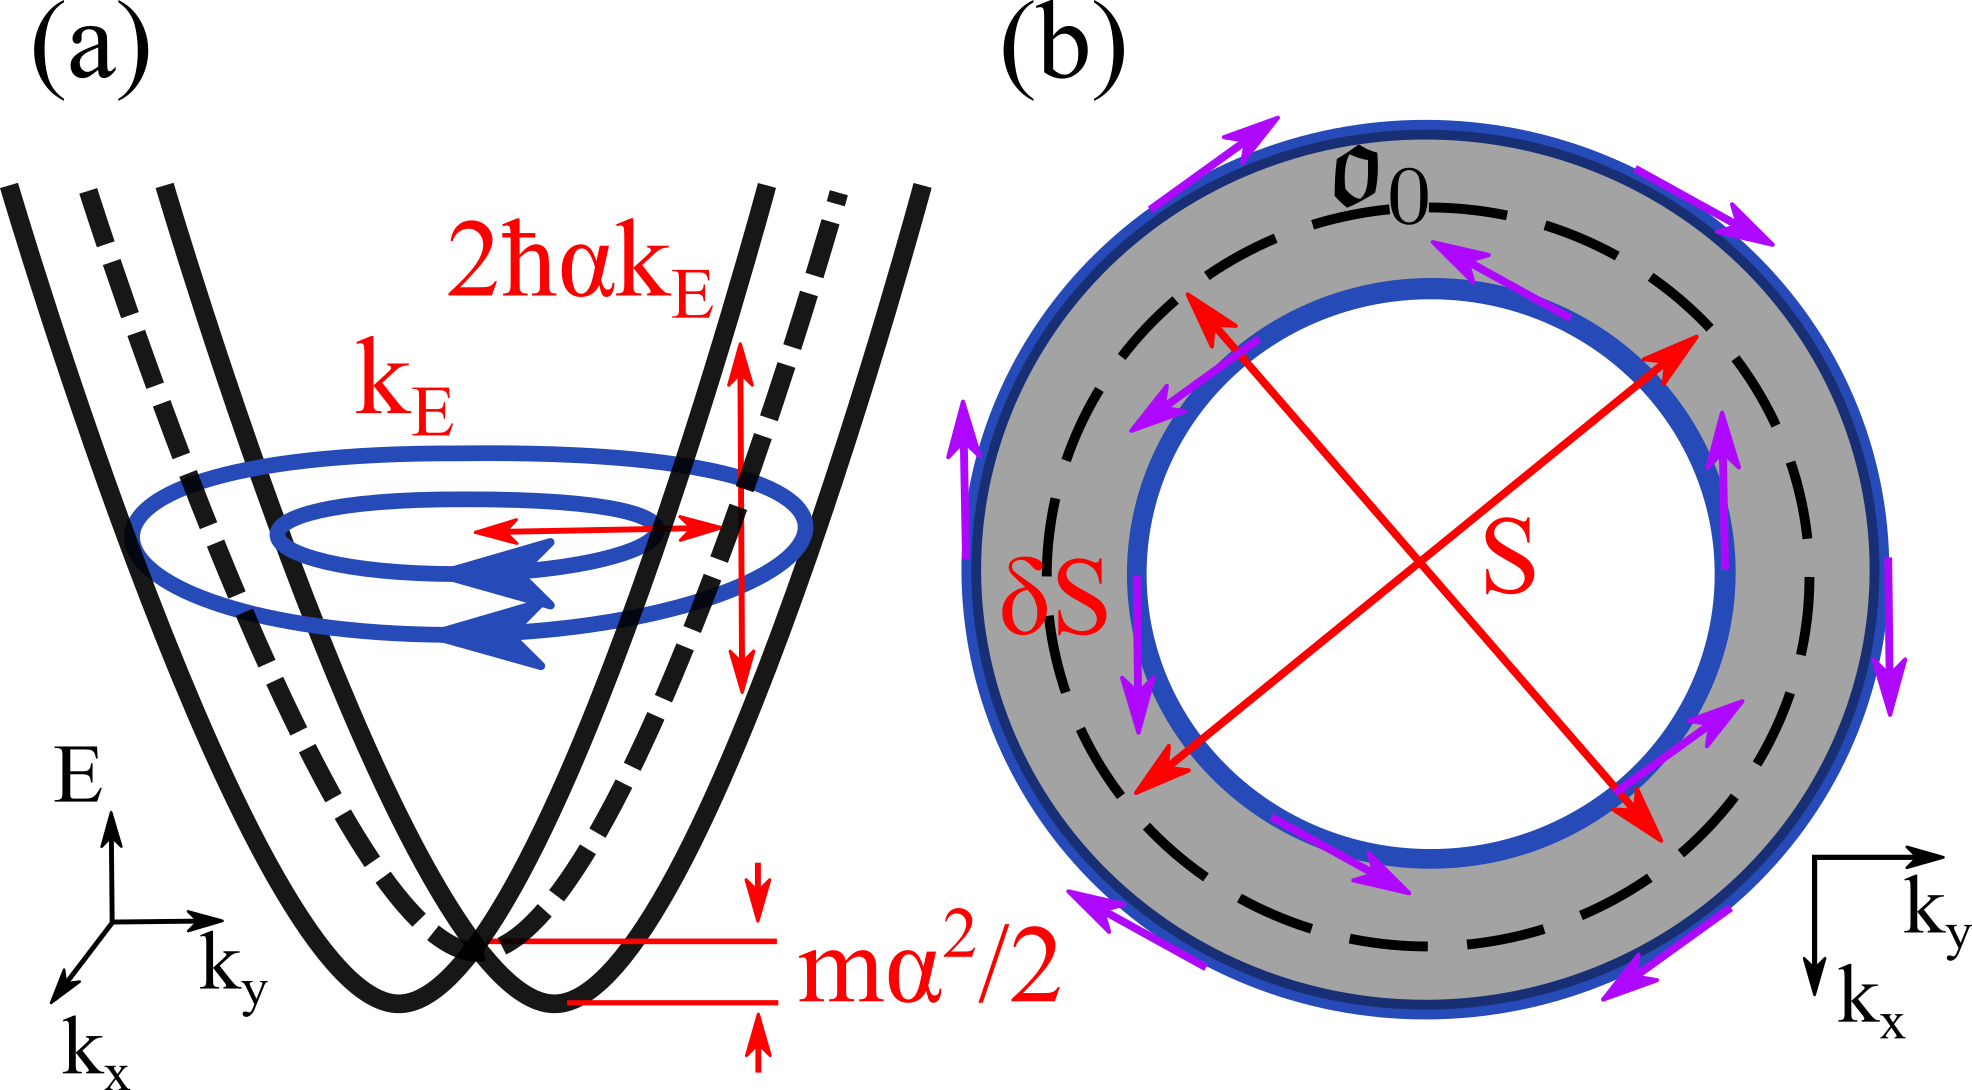
\includegraphics[width=0.8\textwidth]{../figures/orbits.png}
	\centering
	\caption{(a) 实线(虚线)阐释了具有(没有)Rashba自旋轨道耦合的二位电子气的能带色散。图中具有方向的圆代表了磁振子轨道,其中磁场方向为$-z$方向。 (b) 虚的圈$S$标注出了零阶轨道$\frako_0$;$\delta S$是自旋轨道耦合劈裂的轨道的面积之差;紫色的箭头标出了自旋结构。\label{fig:orbits}}
\end{figure}

我们的工作给出了一个适用于近简并能带的推广的量子化条件,这个量子化条件的适用范围包括具有自旋轨道劈裂的能带。我们定义近简并为磁振子面积的差远小于磁振子面积的平均值$|\delta S/S|{\ll}1$。我们提出的量子化条件还依赖于另一个条件:$S$远大于$1/l^2$,这里的$l$事磁长度$l{=}\sqrt{\hbar/eB}$;这个条件也是标准的准经典Onsager-Lifshitz-Roth理论假设。通过引入两个小量$|\delta S/S|$和$1/l^2|S|$,我们的研究推广深化了前人仅仅基于一个小量的准经典理论\cite{kohn_effham,blount_effham,rotheffham,wannier_fredkin,fischbeck_review,Mikitik_quantizationrule,topoferm,100p,gao_zero-field_2017}。

$1/l^2|\delta S|$量化了由塞曼能导致的近简并的轨道的耦合。在$l^2|\delta S|{\gg}1$的情况下,Onsager-Lifshitz{-Roth}量子化条件可以分别作用在两个共心但是不耦合的磁振子轨道。在另外一个极限$l^2|\delta S|{\ll}1$,自旋轨道耦合导致的劈裂可以忽略,我们可以采用已有的严格简并能带的量子化条件\cite{rotheffham,rothmag,topoferm,100p,Mikitik_quantizationrule}。我们的统一的量子化条件给出了介于前述的两个极限情况下的朗道能级的解($l^2|\delta S|{\sim}1$),这种情况下,塞曼能和自旋轨道耦合的能量基本相同;而前人的工作仅仅展示了这两个能量一个远大于另一个的情况下的量子化条件。我们工作给出了在任意对称群的具有自旋轨道耦合的晶体的量子化条件。章节\ref{sec:qtznrules}描述了这个近简并能带的量子化条件,其中哦我们假设了一个自旋二分之一(或者赝自旋二分之一)的自由度。正如章节\ref{sec:discussion}所述,我们的量子化条件能够涵盖任意带数的近简并能带的朗道量子化。


在章节\ref{sec:Rashba}中,我们利用具有Rashba和Dresselhaus自旋轨道耦合的二维电子气,证明了我们的量子化能级的有效性。如果给具有Rashba自旋轨道耦合的二维电子气加上足够强的面内磁场,能带中的Dirac点不仅仅会移动,而且会倾斜,成为一个第二类的狄拉克点\cite{soluyanov_type-ii_2015, muechler_tilted_2016, bergholtz_topology_2015}。在章节\ref{sec:inplanezeeman}中,我们研究了第二类狄拉克点附近的Landau-Zener隧穿现象。特别的,我们将要证明我们的量子化条件囊括了近简并能带之间的量子隧穿,这个现象被称为带间的磁隧穿\cite{kaganov_coherent_1983,slutskin_dynamics_1968,AALG,100p}。我们将要认真研究一个最近提出的二类狄拉克点附近的完美Klein隧穿的现象\cite{obrien_magnetic_2016},我们发现如果考虑了塞曼效应的话,这个完美隧穿永远不会发生。


\section{量子化条件\label{sec:qtznrules}}

首先让我们大致解释一下这个量子化条件是怎么出现的;我们将这个量子化条件的分步的严格的证明留到附录\ref{app:quantizationruleproof}中。我们要考虑的是一个没有加磁场的时候有着离散平移不变性的哈密顿量: $\hat{H}_0{+}\delta \hat{H}$。前面的这个分解要求$\hat{H}_0$的能带在每一个波矢$\bk$处是$D$重简并的,而$\delta \hat{H}$则作为微扰破除这个$D$重简并。简单起见,我们假设$D{=}2$的自旋简并,$D>2$的情形则留在附录\ref{app:quantizationruleproof}中讨论。一个简单的例子是$\hat{H}_0$是薛定谔哈密顿量,而$\delta \hat{H}$是自旋轨道耦合的哈密顿量;另一个例子是$\hat{H}_0$是具有空间反演的包含自旋轨道耦合的泡利哈密顿量,而$\delta \hat{H}$是一个晶格畸变,轻微破坏了空间反演对称性。

现在让我们加上一个磁场,我们首先考虑忽略$\delta \hat{H}$和塞曼效应的自旋简并的朗道能级。在准经典的描述下,我们对$\hat{H}_0$的低能简并的能带的磁场动力学性质进行考察,这条能带的色散记为$\var(\bk)$。比如说,对于Rashba模型,$\var(\bk){=}\hbar^2 k^2/2m{+}\order(k^4)$。众所周知,朗道量子化是由Peierls修正得到的$\var(\bk){\rightarrow}\var(\bK)$\cite{peierls_substitution},这里的$\boldsymbol{K}{:}{=}\boldsymbol{k}{+}(e/\hbar) \boldsymbol{A}(i\nabla_{\boldsymbol{k}})$,并且$\boldsymbol{A}(\br)$是矢势。我们假设磁场沿着$-z$方向,$[K_x,K_y]{=}i\lmt$。准经典的波函数的解对应着电子在$\var(\bk)$的等能面作回旋运动【见图\ref{fig:orbits}(b)】,这个蕴含着电子运动方向(运动方程为$ \hbar dk_{\alpha}/dt {=} \lmt \epsilon_{\ab}\partial \var/\partial k_{\beta} $,其中 $\epsilon_{xy}{=}{-}\epsilon_{yx}{=}1$)的轨道被称为零阶轨道$\frako_0$。在这个工作中,我们仅仅关注闭合的轨道,闭合的意思指的是轨道不会横穿布里渊区。

朗道能级的量子化条件反映了WKB准经典波函数在轨道$\frako_0$上的单值性\cite{berry_mount_review},换句话说,电子在一个磁振子周期$T_c$中获得的相位是$2\pi$的整数倍:$(l^2S(E){+}\gamma)/2\pi{\in}\Z$。最高阶的相位是是$l^2S{:}{=}{-}l^2\int_{0}^{T_c} k_x \dot{k}_y dt$;$S$同时也可以阐释为具有正负号(对于电子型的轨道是正的)的$\bk$空间$\frako_0$的面积,见图\ref{fig:orbits}(b)。$\gamma$是第二阶的Maslov相位修正\cite{keller1958},这个修正等于$\frako_0$绕的圈数$r$乘以$\pi$,也就是切向量的绕圈数)\cite{100p};对于一个能够连续变化为圆的轨道,$r{=}{\pm} 1$。在零阶近似下,所有的朗道能级是自旋简并的,能级间隔是
\e{ \var_c:=\f{2\pi}{l^2|\partial S/\partial E|}:=\f{\hbar^2}{ml^2}:=\f{h}{T_c}. \label{def:cyclotron}}
这里,$\var_c$和$T_c$分别是零阶轨道的磁振子能量和周期,$m$是有效质量。下面开始,朗道能级的简并指的就是自旋简并。



当我们考虑一阶效应的时候,$\delta \hat{H}$和塞曼效应会导致一个一阶的相位修正($\lambda_a$),这个相位修正一般而言对两个不同的自旋态是不同的(我们用$a{=}1,2$标记):
\begin{equation}
l^2S(E)+\lambda_a(E,B)+\gamma=2\pi n,\as  n\in \mathbb{Z},\;a=1,2. \label{eq:rule}
\end{equation}
这表示朗道能级的自旋简并被破除,朗道能级之间的间隔是$\var_c|\lambda_1{-}\lambda_2|/2\pi$。相位修正$\lambda_a$可以看成一个时间周期性的,微扰性的哈密顿量($\calh$)的Floquet准能量\cite{shirley_solution_1965},这个哈密顿量控制着自旋波函数的演化。$\lambda_a$是下面路径有序的指数积分的本征值$\{e^{i\lambda_a}\}_{a=1}^2$:
\begin{equation}
\A{:}{=}\overline{\exp}\left[-\frac{i}{\hbar}\int_0^{T_c} \calh(\bk(t)) dt\right],
\label{eq:prop}
\end{equation}
这里$\bk(t){\in}\frako_0$是一个时间周期性的函数,由运动方程决定。$\calh$是一个$2\times 2$的矩阵:
\begin{equation}
\calh=\delta \var +B\bigg(M_z -g_s\mu_{B}\f{s_z}{\hbar} + e\epsilon_{\alpha\beta}\mathfrak{X}_{\beta}v_{\alpha}\bigg):=\delta \var+B\calm,\label{eq:H1}
\end{equation}
$\delta \var$是$\delta \hat{H}$在$\hat{H}_0$的简并子空间(也就是前述的两条简并的带)中的投影。出于简单起见,我们假设$\delta \var$的迹是零;如果 $\delta\hat{H}$是一个自旋轨道耦合的哈密顿量,那么$\delta \var$的迹是零是得到保证的。更一般的情况下,我们总可以将$\delta \hat{H}$的投影的有迹的部分吸收到$\var(\bk)$的定义里去。在劈开的能带里(我们将这两个能带标记为${+}$和$-$,其中$+$是外面的轨道,$-$是里面的轨道),$\delta \var$是一个对角的矩阵,其对角元($\delta \var_+,~\delta \var_-{=}{-}\delta \var_+$)和耦合参数相关
\e{-\int_0^{T_c} (\delta \var_+{-}\delta \var_-) \frac{dt}{\hbar} \approx l^2\delta S. \label{spinsplitwkb}}

式\ref{eq:H1}中剩下的项可以看成一个广义的塞曼作用项$B\calm$,这一项正比于$B$,是Peierls-Onsager哈密顿量$\var(\bK)$的一阶修正\cite{rotheffham,blount_effham,kohn_effham}。这个广义的塞曼作用项包括近简并能带的自旋的塞曼作用能($g_s\mu_Bs_z/\hbar$)和轨道磁矩($M_z$)的塞曼作用能\cite{thonhauser_orbital_2005};轨道磁矩可以用布洛赫波$\psi_{n\bk}$之间的速度矩阵元表示出来$\boldsymbol{\Pi}_{mn}=i\langle\psi_m|[\hat{H}_0, \hat{\boldsymbol{r}}]|\psi_n\rangle/\hbar$:

\e{
	[M_z]_{mn}=\f{ie\hbar}{2}\sum_l'\f{\Pi_{x,ml}\Pi_{y,ln}-\Pi_{y,ml}\Pi_{x,ln}}{\epsilon_m-\epsilon_l}. \label{eq:orbitalmoment}
}
这里,对$l$的求和不包括这两条近简并的能带。最后,广义的塞曼作用项还包括一个几何相位的贡献,这一个贡献可以用$2\times 2$的非阿贝尔的贝里联络\cite{berry_quantal_1984,wilczek_appearance_1984}和零阶的能带速度表达出来
\e{\mathfrak{X}_{\beta,mn}{=}i\braket{u_m}{\partial u_n/\partial k_{\beta}},  \;\;\;v_{\alpha}:= \f{1}{\hbar}\p{\var}{k_{\alpha}},\label{berryconn}}
这里$\{u_n\}_{n=1}^2$是布洛赫波的周期性部分。

式\ref{eq:rule}至\ref{berryconn}能够让我们将$\lambda_{1,2}$计算到$1/l^2|S|$和$|\delta S/S|$的最低阶,这些式子对任意有限的$l^2|\delta S|$和$|B\calm|/\delta \var_{\pm}$都是有效的。值得指出的式,我们提出的量子化条件相对于近简并能带构成的子空间内的幺正变换是不变的(见附录\ref{app:quantizationruleproof})。在下面的讨论中,如果可能的话,有的时候采用一个和$\bk$无关的基来表达$\calh$更加方便,这种情况下,非阿贝尔的贝里联络这组基下面为零。

\subsection{在两种极限情况下恢复到Onsager-Lifshitz量子化条件}\label{sec:recoveronsager}

现在,我们用近简并的能带(用$\pm$标志)作基,讨论一下$\delta \var$和$B\calm$相互之间的大小关系。我们将要证明,在其中一个远大于另外一个的情况下,我们提出的量子化条件会恢复到已有的针对独立轨道或者简并轨道的Onsager-Lifshitz-Roth量子化条件。

\noi{i} 如果$|\var_+{-}\var_-|$在$\frako_0$的每一个点都远大于$B|\calm_{+-}|$。在这样的情况下,电子在磁场下将会进行绝热(也就是维持在同一个能带的)运动\cite{nenciu_review},此时两个轨道可以看成非简并并且独立的。在$B{\rightarrow} 0$的情况下,如果两条近简并的能带没有交上的话,电子的运动始终会退化为绝热运动。(有的时候近简并的能带会交上,一个例子就是二类狄拉克点,这个例子将在小节\ref{sec:inplanezeeman}和小节\ref{sec:rotsymmbreakdown})在这样的情况下,我们可以忽略带间跃迁的矩阵元$B\calm_{+-}$,此时$\cala$成为一个对角的矩阵,对角元$e^{i\lambda_{\pm}}$为
\e{\lambda_{\sma{\pm}} = -\int_0^{T_c}\calh_{\sma{\pm\pm}}\f{dt}{\hbar}=\pm \f{1}{2}l^2\delta S - B\int_0^{T_c}\calm_{\sma{\pm\pm}}\f{dt}{\hbar}.  \label{phaseindependentorbit}}
式\ref{eq:rule},以及式\ref{phaseindependentorbit},和前人的针对独立,非简并的面积为$S{\pm}\delta S$的两个轨道的Onsager-Lifshitz量子化条件是一致的\cite{Onsager,lifshitz_kosevich,lifshitz_kosevich_jetp}。这个独立轨道的量子化条件包含了首先由Roth\cite{rothmag}提出的相位修正。如果我们微扰地加进$B\calm_{\sma{+-}}$,$\lambda_{\pm}$ (参见 式\ref{phaseindependentorbit})可以表达为$B$地洛朗级数,并且最低阶项时$1/B$;这一点将会在下面地样例讨论(参见式 \ref{lambdasmallB})中设计,并且会被用来解释量子振荡的多种现象(参见节\ref{sec:qo})。


\noi{ii} 让我们现在讨论广义的塞曼能$B\calm$远大于$(\delta \var_+{-}\delta\var_-)$的情况。式\ref{eq:rule}至\ref{berryconn}以及$\calh{\approx}B\calm$,和我们之前的工作中\cite{topoferm,100p}得到的任意对称性的简并轨道的量子化条件是一致的。


由式\ref{eq:rule}至\ref{berryconn}总结出来的量子化条件,是本章的理论性的进展,本章下面的内容主要关注这个量子化条件会带来什么样的物理现象。我们首先要在绝热近似失效的时候(也就是$\delta \epsilon$和$B\calm$的大小相互竞争的时候)证明我们的量子化条件的有效性,这包括两种情况:(i)如果自旋劈裂的轨道在连续旋转变换下不变(比如说Rashba二维电子气模型),那么绝热近似在整个轨道都会失效(参见节\ref{sec:Rashba})。(ii)如果自旋劈裂的轨道是不对称的,绝热近似有可能在某一个孤立的点失效,一个简单的例子就是能带在第二类狄拉克点处相交(参见节\ref{sec:inplanezeeman})。在节\ref{sec:llquasideg}中,我们将要讨论多少个实的参数才能够调节得到$\lambda_1{=}\lambda_2$(mod $2\pi$),这个式子等价于朗道能级的近简并。


\section{案例研究:任意方向磁场中的Rashba二维电子气}

\subsection{面外磁场中的Rashba二维电子气}\label{sec:Rashba}

在这一节里,我们将要将我们的量子化条件应用于Rashba模型(参见式\ref{eq:Rashba-Hamiltonian}),这种情况下,简单的解析的朗道能级的解式存在的,可以和我们的量子化条件做对比\cite{bychkov_oscillatory_1984}。

出于简单起见,我们认为式\ref{eq:Rashba-Hamiltonian}中的泡利矩阵对应的就是自旋:$s_i{=}\hbar \sigma_i/2$。我们来计算半径为$k$的磁振子轨道$\frako_0$上的有效哈密顿量$\calh(\bk)$。用Rashba哈密顿量$H_R$(参见式\ref{eq:Rashba-Hamiltonian})的能带作基
\e{\calh(\bk)=-\hbar\alpha k\tau_z{+}\f{g_{s\perp}}{2}\mu_{\sma{B}}B\tau_x {-} \f{eB\hbar}{2m} (\tau_x-I) \epsilon_{\alpha\beta} k_{\alpha}\nabla_{\beta}\theta,\label{rashbaeffham}}
这里$\tau_i$是一套新的泡利矩阵,$\tau_z{=}{+} 1$ 和 ${-}1$ 分别对应的是外轨道和内轨道。 $e^{i\theta_{\bk}}{=}(ik_x{-}k_y)/k$是面内的$H_R$的自旋劈裂场$(-\hbar\alpha k_y,\hbar\alpha k_x,0)$的角度(参见式 \ref{eq:Rashba-Hamiltonian}),这个自旋劈裂场在$\frako_0$上转了一圈;由于我们基的自旋平行(或者反平行)于自旋劈裂场,因此也转了一圈【参见图\ref{fig:orbits}(b)】。上式中正比如自旋旋转速度($\nabk \theta$)的项来自于非阿贝尔的贝里联络。$\calh$的第一项对应于自旋轨道耦合引起的劈裂;其余项可以认为是磁场导致的能带变形。轨道磁矩$B M_z$一般而言会混合近简并的两个带和其余的所有能带,在这里这个效应被吸收在有效的$g$因子中$g_{s\perp}$。众所周知,塞曼效应一般会让自旋朝向磁场$\bB$的方向;令人惊异的是,非阿贝尔的贝里相位在这里也有一个自旋极化的效应,但是和塞曼效应方向相反。这两个效应在自由电子的时候完全抵消($g_{s\perp}=2$以及 $m$等于自由电子质量$m_0$),这个抵消一般不发生在能带电子上。

由于$H_R$的连续旋转对称性的存在,$\nabk \theta$的大小是$1/k$,并且和$\frako_0$相切;因此,$\calh$在$\frako_0$上是一个常数,而传播子则化简为不需要路径有序的$\cala{=}e^{{-}i\calh T_c/\hbar}$,因此量子化条件的相位修正仅仅是$\calh$的本征值乘以$T_c$:
\begin{equation}
\lambda_{\pm}=\pm\f1{2}\sqrt{({l^2\delta S})^2+\pi^2(g_{s\perp}m/m_0-2)^2}+\pi. \label{eq:Rashba-lambda}
\end{equation}
这是一个面积差$\delta S$(参见式\ref{deltaSvsS})和有效质量$m$的函数。多出来的$\pi$来自于单带的贝里相位,体现在$\theta_{\bk}$绕了${\pm}2\pi$。两个在根号下面的量来自于自旋轨道耦合导致的轨道劈裂$\delta \var$以及(在零场的能带基下的)$B\calm$的带间矩阵元。

在弱耦合极限下,$l^2\delta S \gg \pi|g_{s\perp} m/m_0{-}2|$,我们可以将式\ref{eq:Rashba-lambda}展开为$B$的洛朗级数:
\e{\lambda_{\pm}= \pm \f{l^2\delta S}{2} +\pi \pm \f{\pi^2}{4}\f{(g_{s\perp}m/m_0-2)^2}{l^2\delta S} + O(B^2). \label{lambdasmallB}}
式\ref{eq:rule}以及式\ref{lambdasmallB}的右手边前两项,也可以从标准的针对独立轨道的Onsager-Lifshitz量子化条件导出,其中$\pi$来自于贝里相位的修正:$l^2(S{\pm}\delta S)/2\pi {\in}\Z$。更高阶的项则来自于磁场导致的能带之间的混合。Mineev在Rashba模型下得到了式\ref{lambdasmallB}中的一部分\cite{mineev_haas--van_2005};由于没有考虑带间的贝里联络,他漏掉了$(g_{s\perp}m/m_0-2)$中的第二项(参见式\ref{lambdasmallB})。

在强耦合极限,也就是$l^2\delta S {\ll}\pi(g_{s\perp}m/m_0{-}2)$的情况下,$\lambda_{\pm}{\approx}{\pm}\pi g_{s\perp}m/2m_0$ mod $2\pi$,这对应着没有自旋轨道耦合的情况下,朗道能级劈裂了$g_{s}\mu_BB$。

我们的量子化条件【式\ref{eq:rule}和\ref{eq:Rashba-lambda}】可以和已知的Peierls替换过的哈密顿量(加上自旋塞曼效应)的精确解进行比对。精确解\cite{bychkov_oscillatory_1984}可以通过下式得出:
\e{
	&n_{\pm}=\frac{l^2S}{2\pi}+\frac{l^2\delta S}{16\pi}\f{\delta S}{S}\lin 
	&\pm\f1{2}\sqrt{\bigg(\frac{l^2\delta S}{8\pi}\f{\delta S}{S}\bigg)^2+(l^2\delta S)^2+\pi^2\bigg(\f{g_{s\perp}m}{m_0}-2\bigg)^2},\label{eq:Rashba-exact}}
这里的$\delta S(E)$和$S(E)$的形式参见式\ref{deltaSvsS};$n_{+}{\ge} 1$和$n_-{\ge} 0$是整数的朗道能级的标号,$\pm$代表两套朗道能级。在近简并的($\delta S/S\ll 1$)准经典的($1/l^2S \ll 1$)情况下,在$l^2\delta S$是有限的时候,式\ref{eq:Rashba-exact}里面的$\delta S/S$项可以忽略,于是式\ref{eq:Rashba-exact}就退化为我们的量子化条件,其中$\lambda_{\pm}$由是\ref{eq:Rashba-lambda}给出。


我们进一步给$H_R$加上Dresselhaus自旋轨道耦合,在这样的情况下,据我们所知,朗道能级的严格解析解是不存在的。这种情况下,我们可以通过数值对角化来验证我们的量子化条件的可靠性,这一部分内容在附录\ref{app:approximatevsexact}中。

\subsection{磁隧穿的案例研究:倾斜磁场中的Rashba二维电子气}\label{sec:inplanezeeman}

我们的下一个案例研究是一个(接近)相交的二类狄拉克点\cite{soluyanov_type-ii_2015,muechler_tilted_2016}。二类狄拉克点是传统狄拉克点的一个变种,其区别在于二类狄拉克点的能带色散不是对称的。在二类狄拉克点附近的量子隧穿数学上和Landau-Zener隧穿是一致的,仅仅是电场力变成了洛伦兹力\cite{AALG,obrien_magnetic_2016,kane_blount}。这里,我们将要证明Landau-Zener动力学很自然的可以从我们的量子化条件得出(式\ref{eq:rule}到式\ref{eq:H1})我们将要研究电子的运动会怎么受到塞曼效应的影响。特别地,我们将会展示O'Brien等人预言的\cite{obrien_magnetic_2016}完美的Klein透射在考虑进塞曼效应之后,并不是真正地完美。

我们再次从Rashba模型出发(参见式\ref{eq:Rashba-Hamiltonian}),它有一个旋转对称的狄拉克点。要将这个狄拉克点变成二类的,我们引入一个面内的磁场$B_\parallel$(平行于$y$方向)导致的塞曼项:
\e{ 
	H_{RZ}=\f{{\hbar^2}k^{2}}{2m}+\delta \var; \;\;\;\delta \var=d_x\sigma_x+d_y\sigma_y,\lin
	(d_x,d_y):=(-\hbar\alpha k_y,\hbar\alpha k_x+\zpar),\;\;\;\zpar:= g_{s\parallel} \mu_B B_{\parallel}/2.
	\label{eq:RZ-Hamiltonian}}
尽管这一项同时破坏了时间反演($T$)和二重旋转($\rot_2$),他们的乘积($\rot_2 T$)还是哈密顿量的对称性,这一点体现在 $\sigma_x H^*_{RZ}(\bk)\sigma_x{=}H_{RZ}(\bk)$, 并且让每个$\bk$的自旋严格躺在面内。二维情况下,在这个对称群中,狄拉克点可以移动,但是不能够打开能隙。面内的塞曼场不仅挪动了狄拉克点的位置到
\begin{eqnarray}
\bar{k}_x & = & -\frac{\zpar}{\hbar\alpha},\;\bar{k}_y=0,\;\epsilon_{0}=\frac{\zpar^{2}}{2m\alpha^2},\label{whereisdiracpoint}
\end{eqnarray}
而且将狄拉克点的能带倾斜了过来。如果我们在狄拉克点附近线性化这个哈密顿量,我们就可以看到这个倾斜
\e{
	H & =\hbar\alpha\left[\left(\sigma_y-\frac{\zpar}{m\alpha^2}\right)\delta k_{x}-\sigma_{x}\delta k_{y}\right]+\epsilon_{0}.}
当$|\zpar|>|m\alpha^2|$的时候,狄拉克锥在$x$方向倾斜角度超过了90度,进而导致等能线的Lifshitz相变。在线性近似下,等能线从圆形变成了双曲线,这一点体现在图\ref{fig:RZ}(a)中。一个倾斜超过九十度的狄拉克锥就是第二类的狄拉克锥。我们的案例研究就是要研究两个电子口袋连接在一起的第二类狄拉克点(参见图\ref{fig:RZ}(a,b)),这个案例研究和前人的不同\cite{obrien_magnetic_2016,AALG},前人研究的第二类狄拉克点是电子和空穴口袋之间相交得到的。

\begin{figure}
	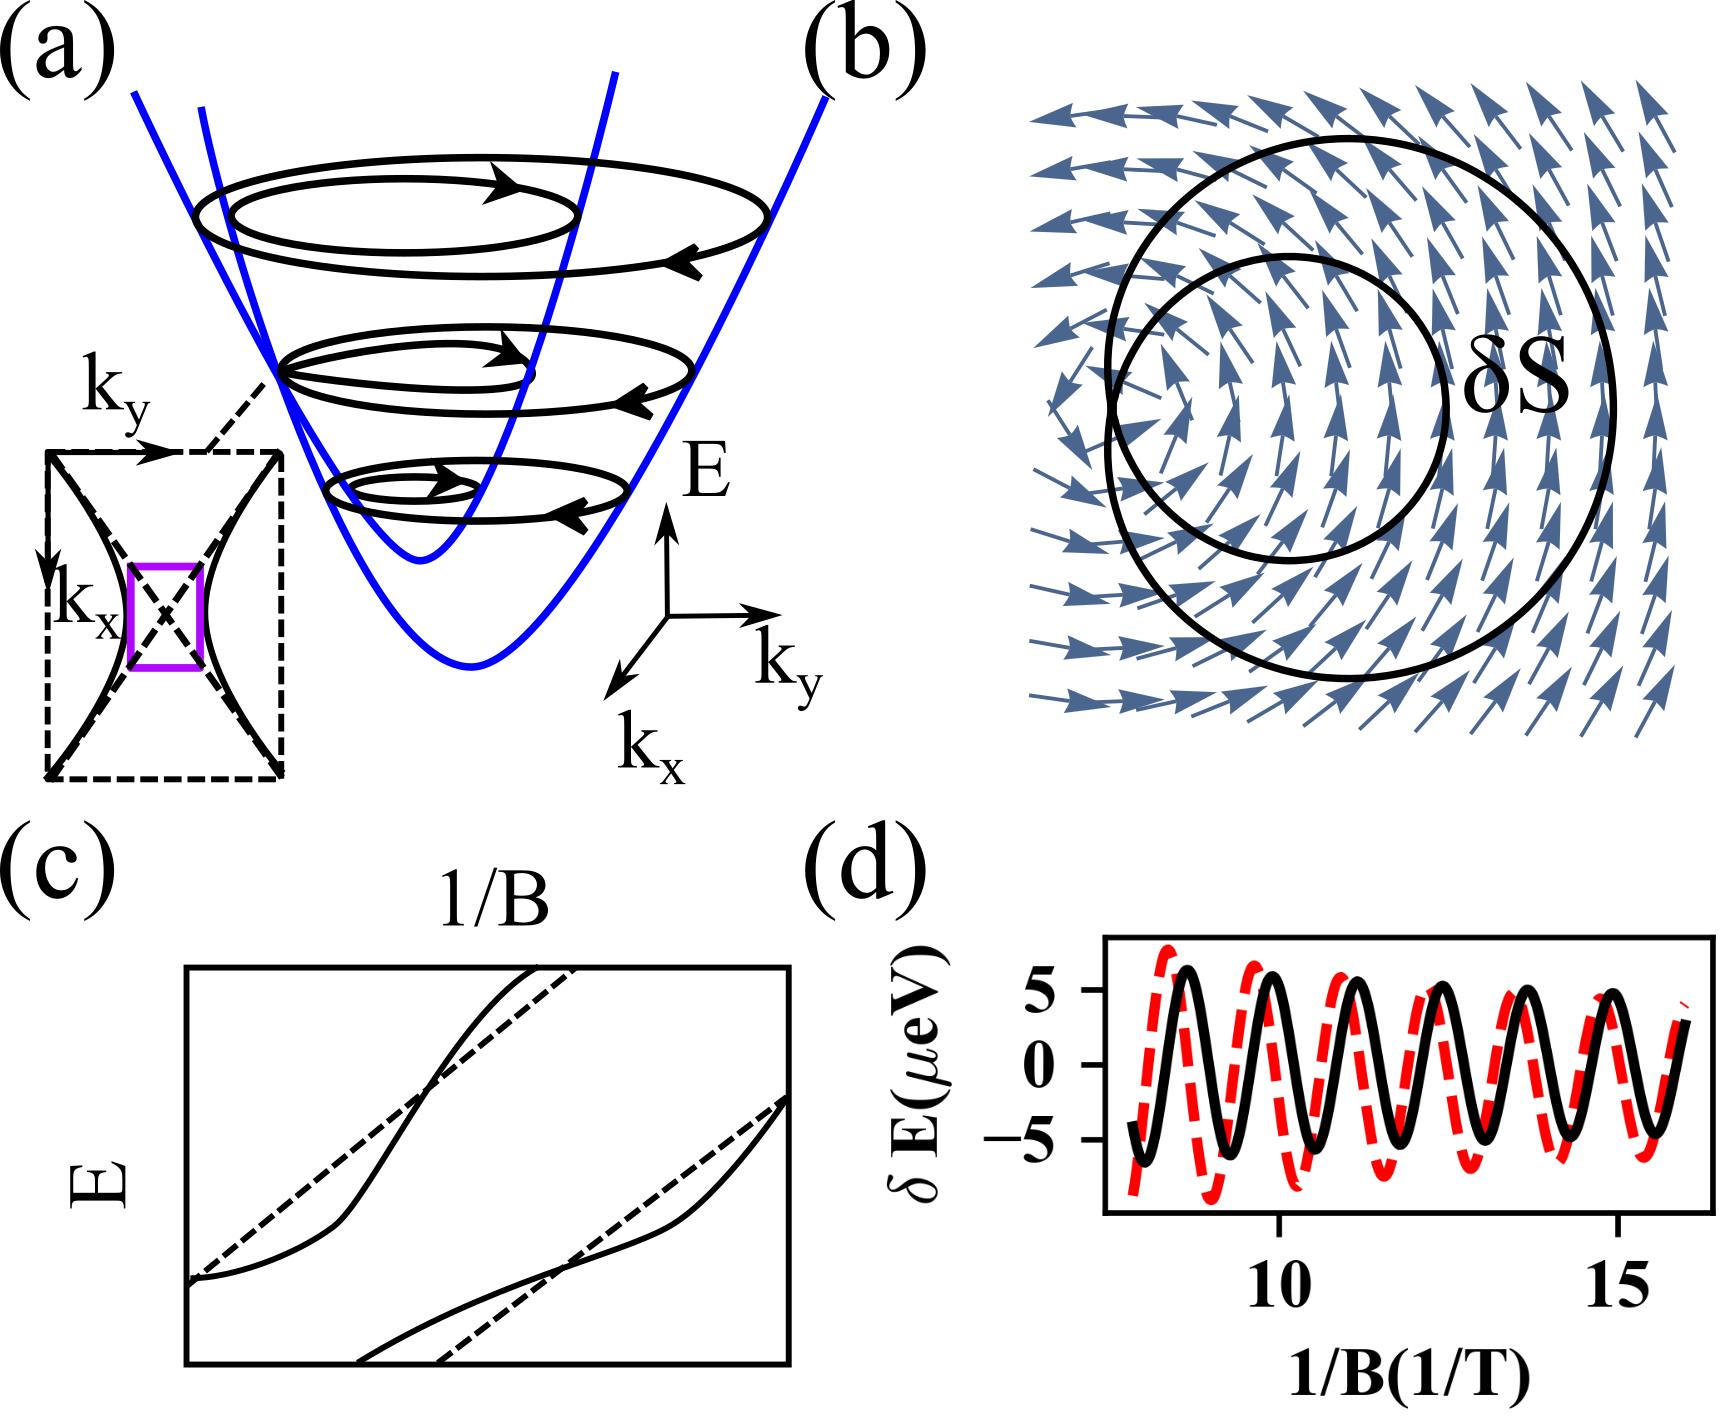
\includegraphics[width=0.8\columnwidth]{../figures/RZ.png}
	\centering
	\caption{(a)展示了Rashba二维电子气在倾斜磁场中的磁振子轨道。内嵌的图展示了第二类狄拉克点的放大图。(b)展示了能量正好在第二类狄拉克点的时候的磁振子轨道。一个能够Klein透射的电子将会沿着这个莫比乌斯环形的轨道运动。这个图片的背景是自旋劈裂场的方向($d_x,d_y$),自旋劈裂场导致了原先的能带$\delta\var$的能量劈裂(参见式\ref{eq:RZ-Hamiltonian}。内(外)圈的波函数的自旋是平行于(反平行于)自选劈裂场的。(c)在弱耦合情况下,演示了在第二类狄拉克点附近的朗道能级。虚线是莫比乌斯轨道的Onsager-Lifshitz-Roth量子化能级(参见式\ref{trefoilrule}),实线则包含了隧穿导致的的一阶修正(参见式\ref{RZfirstorderE}) (d) 黑色的实线是$\delta E_n$(参见式\ref{RZfirstorderE}),也就是由于不是完美Klein透射导致的能量修正;作为对比,红色的虚线是数值严格对角化得到的相应的能量修正。这个图采用了最接近0.45eV的朗道能级,并且采用了偶数$n$;在我们采用的参数下 ($m{=}0.076m_0$, $\alpha{=} 1.5\times10^{5}$cm/s, $Z_\parallel {=}$1meV 以及 $g_{s\perp}=2$),二类狄拉克点在 0.5eV处。 
	\label{fig:RZ}}
\end{figure}

在面内的磁场以外,我们再加入一个面外的磁场$B_{\perp}$,其磁长度为$\lper{=}\sqrt{\hbar/eB_{\perp}}$,磁振子能量为$\var^{\sma{\perp}}_c{:}{=}\hbar^2/m\lper^2{:}{=}\hbar \omega_c^{\sma{\perp}}{:}{=}h/T_c^{\sma{\perp}}$,自旋塞曼效应为$\zper{:}{=}{g_{s\perp}}\mu_B B_{\perp}/2$。我们在这里假设$1/\lper^2S{\ll}1$,这里$S$是零阶轨道(有效质量为$m$半径为$k_E{=}\sqrt{2mE}/\hbar$)。对于远高于$m\alpha^2$和 $\zpar$的能量,近简并条件($\delta S/S{\ll}1$)是满足的,这里$\delta S$是自旋轨道和耦合和面内的塞曼场导致的磁振子轨道的面积差(参见图\ref{fig:RZ}(b))。由于$1/\lper^2S$和$\delta S/S$很小($\lper^2\delta S$是有限的),我们的量子化条件(参见式\ref{eq:rule}至式\ref{eq:H1})可以应用于这个模型,其有效哈密顿量为
\begin{equation}
\calh(t)=\hbar\alpha(k_{x}\sigma_{y}-k_{y}\sigma_{x})+Z_\parallel\sigma_{y}-Z_\perp\sigma_{z}.\label{calHRZ}
\end{equation}
这里,$t$是一个参数化零阶轨道的参数$\bk(t){=}({-}k_E \cos \omega_c^{\sma{\perp}} t, k_E \sin \omega_c^{\sma{\perp}} t)$,在和是\ref{calHRZ}动量无关的自旋基矢下,式\ref{eq:H1}中的非阿贝尔的贝里联络$\mathfrak{X}$为零,因此广义的塞曼作用$B_{\sma{\perp}}\calm$退化为对自旋的塞曼作用$Z_\perp\sigma_{z}$。

正如节\ref{sec:qtznrules}所述,如果两个轨道在一个二类狄拉克点相交,那么绝热极限是不存在的。为了研究这个绝热近似是怎么失效的,我们来研究靠近狄拉克点能量($\epsilon_0$)的朗道能级。我们首先关注除了狄拉克点之外,零级轨道$\frako_0$上处处弱耦合的情况。这个条件等价于能量劈裂(参见式\ref{eq:RZ-Hamiltonian})$|\delta \var_+{-}\delta \var_-|$远大于$B_\perp|\calm_{\sma{+-}}|$,也等价于$\hbar\alpha k_{\sma{E}}{\gg}\var_c^\perp$。在狄拉克点附近(此时定义$t{=}0$),研究电子的运动可以采取线性化$\H$的方法,得到
\e{
	\calh = -\hbar\alpha k_{E}\omega^{\sma{\perp}}_c t\,\sigma_x+(Z_\parallel-\alpha k_{E})\sigma_y-Z_\perp\sigma_z,\label{effhamIIDirac}
}
$\sigma_x$的本征矢就是两个非绝热的能级,其特征斜率为$v_d{:}{=}\hbar\alpha k_E\omega^{\sma{\perp}}_c$;在$t{=}0$的时候,由于$\sigma_{y,z}$的存在,两个非绝热能级会耦合,并且打开一个能隙。一般而言,一个非绝热能级隧穿到另一个非绝热能级的概率是$\rho^2{=}\exp(-2\pi\barmu)$,这里的$\barmu{=}{E_g}^2/{2v_d \hbar}$,而$E_g$是能隙\cite{wittig_landauzener_2005,lifshitz_e.m._quantum_1991};在这种情况下
\e{\barmu=\frac{Z_\perp^2+(Z_\parallel-\alpha k_{E})^2}{2\hbar\alpha k_{E}\var^{\sma{\perp}}_c}, \label{mu1}}
这里$2\hbar\alpha k_E$是能量$E$处的自旋轨道劈裂【参见图\ref{fig:orbits}(a)】。在没有考虑面外的自旋塞曼劈裂的情况下($Z_\perp{=}0$),$\bar{\mu}$在狄拉克点的能量为零 -- 也就是会得到一个概率为1的Klein隧穿,这一点是由文献\onlinecite{obrien_magnetic_2016}在另外一个第二类狄拉克点模型中第一次提出的。但是,如果考虑进$Z_\perp$的话,$\bar{\mu}$永远都不会为零,其最小值为$\bar{\mu}_{\sma{\text{min}}}{:}{=} (g_{s\perp} m/m_0)(Z_\perp/4\hbar\alpha k_{E})$,这个式子也是无量纲的有效质量乘以面外塞曼劈裂处以自旋轨道劈裂。这个最小值对于半导体异质结或者重费米子体系可能比较显著(比如对InAs异质结而言,$g_{s\perp}m/m_0{\sim} 1$)。


如果要得到朗道能级,我们不仅仅需要知道隧穿的概率,还需要知道隧穿过去的波函数的相位。这些信息包含在一个散射矩阵中\cite{AALG,kaganov_coherent_1983}
\e{\mathbb{S}=\matrixtwo{\tau e^{i\barphi}}{-\rho}{\rho}{\tau e^{-i\barphi}},\;\rho=e^{-\pi\barmu},\;\tau=\sqrt{1-\rho^{2}}\label{scattmat}}
这是一个将两分量的WKB准经典波函数在Dirac点附近联系在一起的一个矩阵。这个公式是在塞曼修正过的能带作为基写出来的(也就是式\ref{calHRZ}的本征态);$\mathbb{S}$的对角项(非对角项)对应着带内跃迁(带间跃迁)。带内跃迁的相位是 $\barphi{:}{=}\barmu{-}\barmu\ln\barmu{+}\text{arg}[\Gamma(i\barmu)]{+}\pi/4$其中$\Gamma$是$\Gamma$函数。

远离二类狄拉克点的地方,电子将会以绝热演化(保持在同一个能带)的方式运动。将Landau-Zener隧穿和绝热演化结合起来,我们就可以得到下面的传播子:
\e{{\A}= \matrixtwo{\tau e^{i\bar{\varphi}}}{-\rho}{\rho}{\tau e^{-i\bar{\varphi}}} \diagmatrix{e^{i\tilde{\lambda}_-}}{e^{i\tilde{\lambda}_+}}. \label{propinplanezeeman}}
绝热演化的相位$\tilde{\lambda}_{\pm}$是动力学相位${\pm} l^2 \delta S/2$和外轨道($+$)和内轨道($+$)的贝里相位$\phi^B_\pm$之和。在远高于狄拉克点的地方($|E{-}\epsilon_0|{\gg}|Z_{\perp}|$),Zeeman效应可以忽略,无论是外轨道还是内轨道都包含了狄拉克点,因此$\phi_{\pm}^B{\approx}{\pm}\pi$;在远低于狄拉克点的时候,两个轨道都没有包含狄拉克点,因此$\phi_{\pm}^B{\approx}0$;在狄拉克点附近的时候, $\phi_{+}^B$($\phi_{-}^B$)随着能量连续减少(增加),这一点可以从图\ref{fig:blochsphere}中的布洛赫球上看出来。

\begin{figure}
	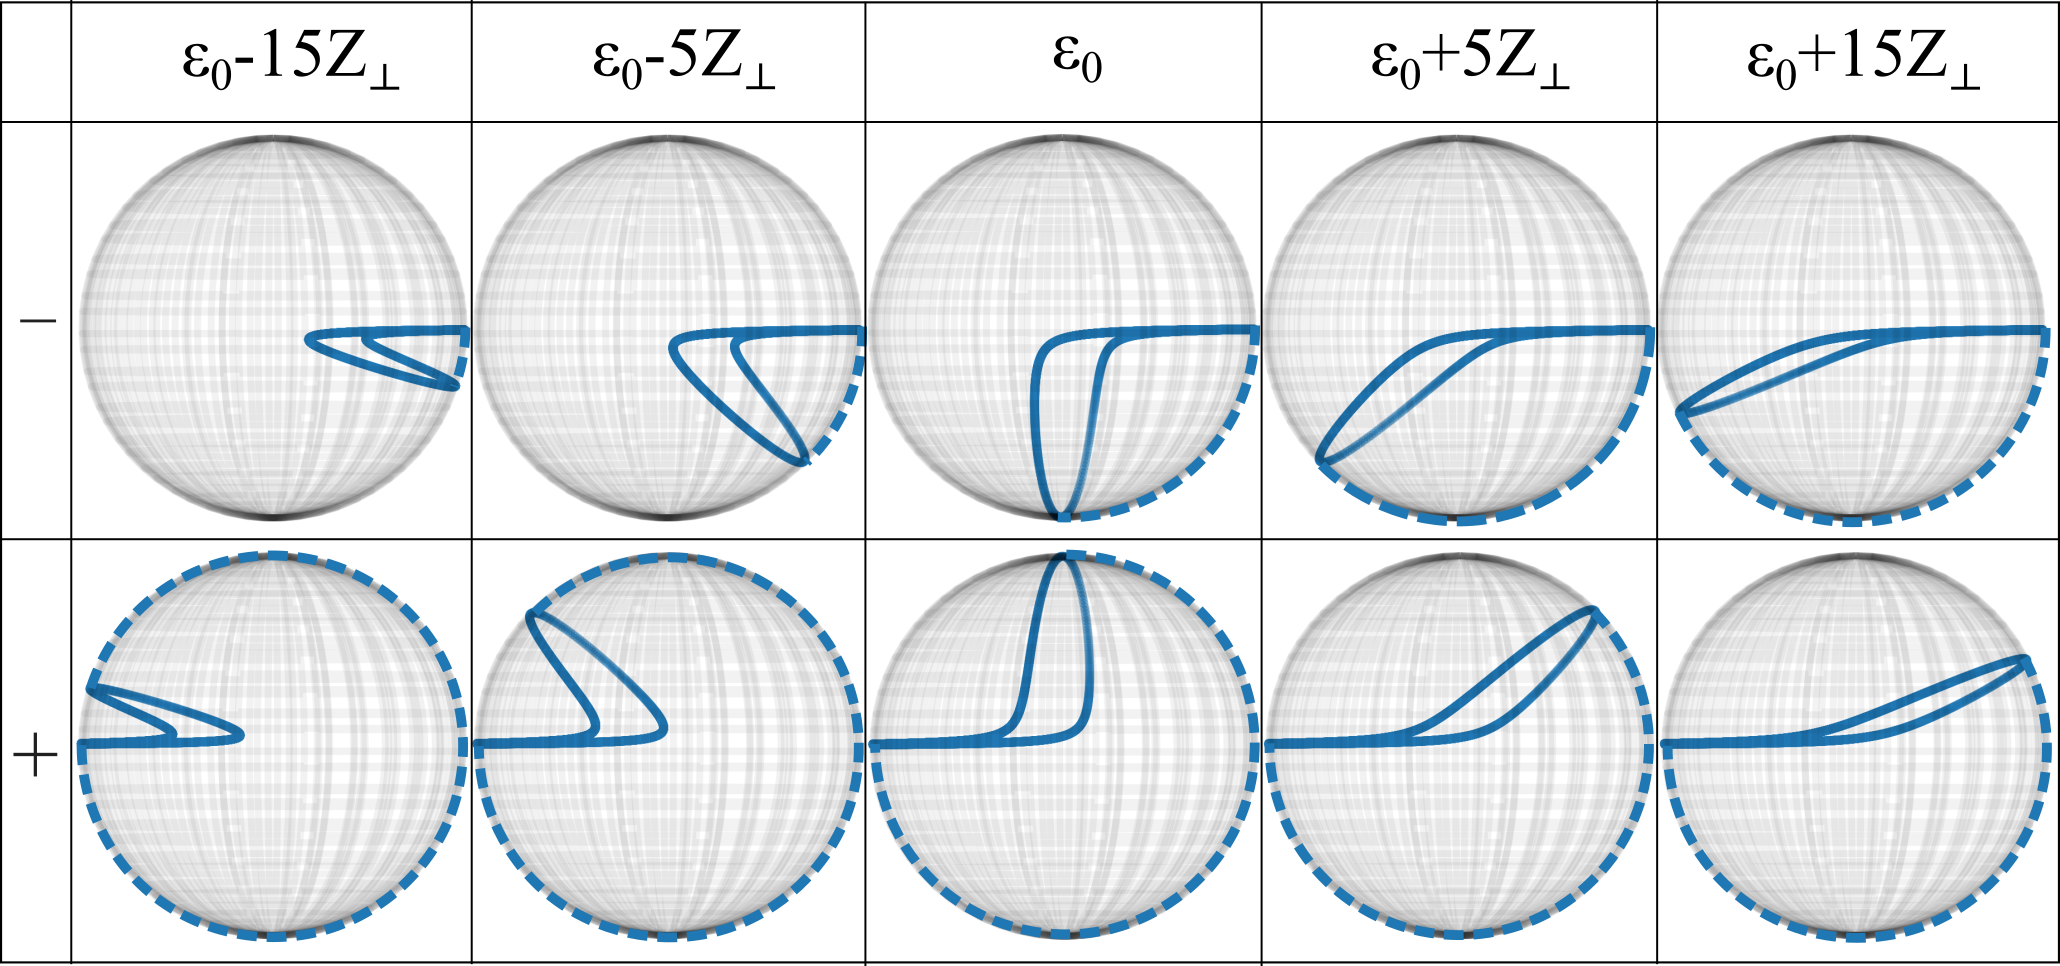
\includegraphics[width=0.8\textwidth]{../figures/blochsphere.png}
	\centering
	\caption{在狄拉克点能量($\epsilon_0$)附近的几个能量出,内轨道(符号是$-$,上排)和外轨道(符号是是$+$,下排)的贝里相位$\phi_{\pm}^B$的立体角表示(参见式\ref{whereisdiracpoint})。在这里,有效哈密顿量(参见式\ref{calHRZ})可以用泡利矩阵分解($\calh{=}\sum_j\calh_j\sigma_j$),这个分解定义了一个三维向量$\boldsymbol{\calh}{=}({-}\alpha k_y$,$\alpha k_x{+}Z_\parallel,{-}Z_\perp)$。$\phi_{\pm}^B$等于${\mp} \boldsymbol{\calh}(\bk)$在$\bk$变化的时候(蓝色的实线)张成的立体角的一半\cite{berry_quantal_1984};立体角的方向由蓝色的虚线表示出来。面外的塞曼场将$\boldsymbol{\calh}$朝向偏出$x-y$平面,但是这个效应仅仅在磁振子轨道的一小部分$(\sim Z_{\perp}/\hbar \alpha k_E)$有明显的贡献。\label{fig:blochsphere}}
\end{figure}

我们的量子化条件(参见式\ref{eq:rule}至\ref{eq:H1}),加上式\ref{propinplanezeeman}中的$\A$的形式,可以简洁地表达为
\e{
	\text{cos}\left[\frac{\Omega_{-}+\Omega_{+}}{2}\right]=\tau\,\text{cos}\left[\frac{\Omega_{-}-\Omega_{+}}{2}+\bar{\varphi}\right], \lin
	\ins{with}\;\Omega_{\pm}=l^2 (S\pm \delta S/2)+\phi_{\pm}^B +\gamma_{\pm}, \label{coscos}
}
$\Omega_{\pm}$是电子在绝热演化穿过$\pm$标志的内外轨道的时候获得的相位;Maslov修正对于圆轨道是$\gamma_{\pm}{=}\pi$。在电子口袋和空穴口袋相交的第二类狄拉克点模型中,也有类似于式\ref{coscos}的量子化条件\cite{AALG}。

在$\bar{\mu}{\rightarrow} \infty$的极限下,Landau-Zener隧穿可以忽略($\tau{\rightarrow}1,\bar{\varphi}{\rightarrow}0$),这个时候式\ref{coscos}简化为两个独立轨道的Onsager-Lifshitz-Roth量子化条件$\Omega_{\pm}/2\pi{\in}\Z$。

对于不为零的磁场,$0{<}\tau{<}1$意味着两个谐频$(\Omega_+{\pm}\Omega_-)$在式\ref{coscos}中会相互竞争,得到一个准随机的朗道能谱\cite{kaganov_coherent_1983}。准随机指的是能谱在磁振子能量的尺度是乱的,但是在更大的尺度上相互关联。要理解这一点,我们将$\tau$看成小量,采用微扰法来分析狄拉克点附近的朗道能级。零阶的情况下,式\ref{coscos}化简为
\e{2l^2S(E_n^0)+\pi = 2\pi n \rightarrow \{E_n^0(B)\}_{n\in\Z}.\label{trefoilrule}}
在到处上面的式子的过程中,我们用到了$\phi^B_-{+}\phi^B_+{=}0$,这一点对于任意的二带模型都是成立的;在图\ref{fig:blochsphere}中,这一点体现在同一能量的两个立体角加和是$4\pi$。式\ref{trefoilrule}可以认为是莫比乌斯轨道的量子化条件,其面积是$2S{=}4\pi m E{/\hbar^2}$;对应的朗道能级(在图\ref{fig:RZ}(c)中画成了实线)相对于$E{\rightarrow}E{+}\pi/l^2(\partial S/\partial E)$和$l^2{\rightarrow}l^2{+}\pi/S$是周期性的。式\ref{trefoilrule}中的$\pi$的相位修正来自于波函数在整个莫比乌斯轨道上的$2\pi$的相位旋转导致的贝里相位,这一点展示在图\ref{fig:RZ}(b)。由于Maslov修正等于$\pi$乘以轨道的绕转数,在这个例子里Maslov修正为$2\pi$。

总结一下,$E_n^0(B)$(参见式\ref{trefoilrule})在小的能量尺度也是周期性的,这个周期性和莫比乌斯轨道的面积有关。如果考虑到Klein透射是非完美的,那么则会个小能量尺度上的周期性就会丢失,但是大能量尺度上的关联始终存在(这个大能量尺度对应着自旋劈裂的轨道之间的面积差$\delta S$),这一点可以从关于$\tau$的一阶修正看出来:
\e{&\delta E_n(B) = \f{(-1)^n}{2\pi} \tau \var_c^\perp \cos\bigg(\f{l^2\delta S}{{2}}+\f{\phi_+^B-\phi_-^B}{2}-\bar{\varphi}\bigg) \lin
	&\approx \f{(-1)^{n+1}m\alpha^2(E-\epsilon_0)(\var_c^{\perp})^{1/2}}{2\sqrt{\pi}\hbar^2
		Z_{\parallel}^{3/2}}\cos\bigg(\f{l^2\delta S}{{2}}-\bar{\varphi}\bigg),\label{RZfirstorderE}}
上式右侧应该在$E{=}E_n^0(B)$计算。第二行开始,我们做了近似$Z_{\perp}{\rightarrow}0$,这个近似在 $g_{s\perp}m{\ll}m_0$的时候是合理的。对于两个相邻的朗道能级,我们在图\ref{fig:RZ}(c)里画出了$E_n^{(0)}+\delta E_n$。图\ref{fig:RZ}(d)中式\ref{RZfirstorderE}和数值对角化比较证明了式\ref{RZfirstorderE}的正确性。

\section{朗道能级的准简并}\label{sec:llquasideg}

\begin{figure}
	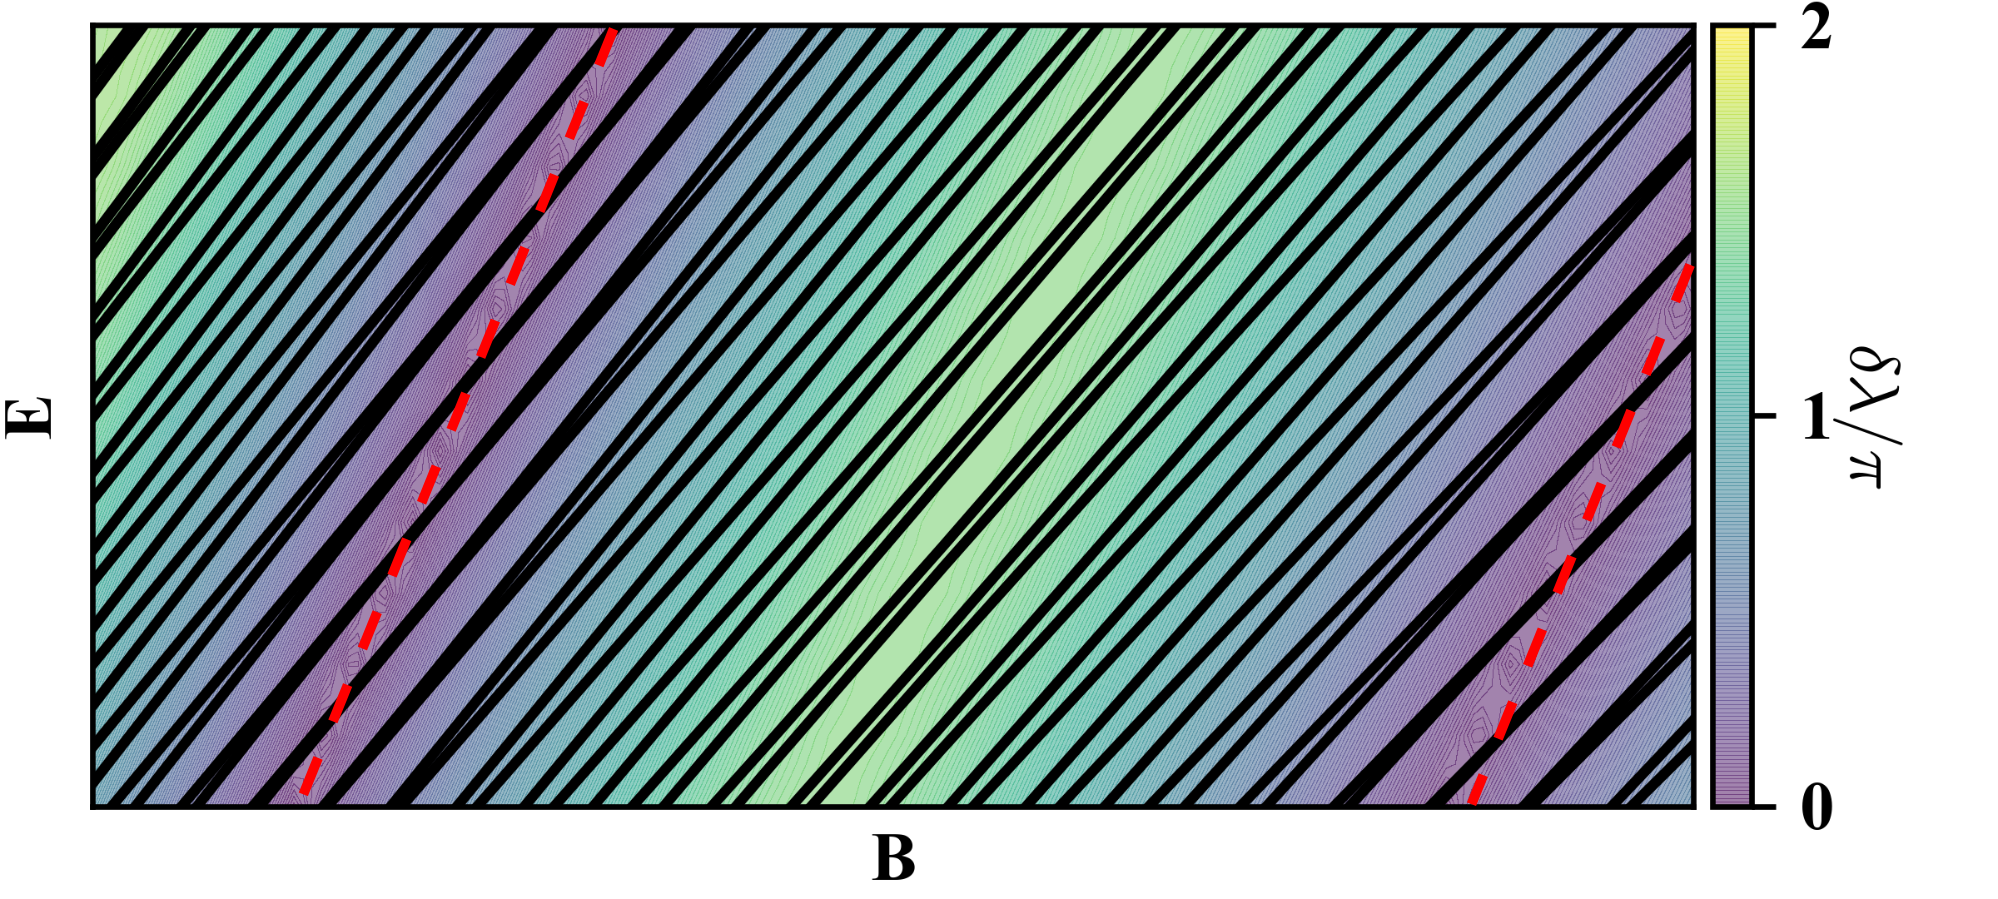
\includegraphics[width=1.0\textwidth]{../figures/LL.png}
	\centering
	\caption{近简并能带中,朗道能级(实线)相对于$B$的色散的一个示意图。背景中的颜色表示的是$\delta\lambda$。当$\delta\lambda\equiv 0\equiv 2\pi$时(用红色的虚线标记),朗道能级就会出现准简并。\label{fig:LL}}
\end{figure}

从式\ref{eq:rule}得到的两套朗道能级一般而言间距是不相等的,而且由于相位修正$\lambda_{1,2}$的存在,一般而言也是不简并的。正如节\ref{sec:qtznrules}所述,两套朗道能级之间的间距近似等于$\var_c\delta \lambda/2\pi$,这里$\delta \lambda=|\lambda_1-\lambda_2|$。反过来,如果$\lambda_1{=}\lambda_2$ (mod $2\pi$),那么朗道能级近似是简并的--这个$\A$的本征值简并的条件需要哈密顿量的一些精细的调节。

在节\ref{sec:relatedegeneracies}中,我们要将$\A$的本征值的简并和朗道能级的(近)简并联系到一起。下一步,我们要解决的问题是多少个实的参数可以调节出$\A$的一个本征值简并时间。对于没有任何对称性的系统,我们的答案是$3$,这一点会在节\ref{sec:introducecodimension}中讨论;如果晶体和轨道存在对称性,那么参数的数目可以减少为$0,1$或者$2$,这一点将会在节\ref{sec:introducecodimension}中讨论。在给出最普适的答案之前,我们将先用两个具有旋转对称性的案例研究(参见节\ref{sec:singleparameterrashba}和\ref{sec:rotsymmbreakdown})来辅助理解,在具有旋转对称性的时候,只需要有一个参数就可以调节得到$\A$的本征值简并,这个参数可以是磁场$B$。

\subsection{$\A$本征值的简并和朗道能级的准简并}\label{sec:relatedegeneracies}


图\ref{fig:LL}展示了一个具有Rashba自旋轨道耦合和Dresselhaus自旋轨道耦合的在近简并区域二维电子气朗道能级的一个示意图。每个量子化条件(参见式\ref{eq:rule})的解,在固定$a\in \{1,2\}$和$n \in \Z$的情况下,在$(E,B)$空间定义了一条线,我们在图中画为实线。而$\A$的本征值简并
\e{\lambda_1(\bar{E},\bar{B})=\lambda_2(\bar{E},\bar{B})+2m\pi, \as m\in \Z \la{eigenvaluedegeneracyA}} 
则定义了另一系列的线(画为红色的虚线)。这个事实仅仅适用于具有旋转对称性的晶体,对于其余的晶体,$\A$的简并点在$(E,B)$空间可能仅仅是一个点或者根本不存在。 这两系列的线(虚线和实线)在离散的点相交,在我们目前的精确度下,这个相交的点就是朗道能级的简并点。原则上来讲,如果朗道能级能够用不同的量子数(比如对称性的本征值)标记,那这个简并点可能是严格的。但是这一个问题目前讨论起来过于复杂,我们留由以后的工作研究。

即使不在这些相交的点,在红色的虚线附近,朗道能级之间的排斥仍然非同寻常的小(我们将要用式\ref{llquasideg}至式\ref{llquasidegB}来量化这一点),这一点可以从图\ref{fig:LL}的紫色部分看出来。对于实验而言,由于无序的存在,严格的简并点和这样的近简并点一般而言没有办法区分\cite{shoenberg_magnetic_2009}。因此,我们要定义一个新的概念:朗道能级的准简并。然后,我们将要搞清楚什么情况下这些准简并点在$(E,B)$空间表示为线,而不是点或者根本没有解。


假设传播子$\A$在$(\bar{E},\bar{B})$处简并【参见式\ref{eigenvaluedegeneracyA}】。一般而言,$(\bar{E},\bar{B})$并不同时式量子化条件的一个解,或者说,一般而言在磁场$\bar{B}$下,$\bar{E}$处一般并没有一个朗道能级。要找到一个朗道能级,我们得调节$E$或者$B$,并且利用$\lambda_{\pm}$是随着$(E,B)$缓慢变化的事实:
\e{l^2\left|\p{S}{E}\right| \gg \left|\p{\lambda_a}{E}\right|,\, \left|S\right| \gg \left|\p{\lambda_a}{l^2}\right|;} 
上述的不等式来自于近简并条件($\delta S{\ll}S$)以及$S(E)$的连续性,具体的证明在附录\ref{sec:proofLLquasideg}。对于一个固定的$\bar{B}$,我们就能在$\bar{E}$附近找到一对靠的非常近的朗道能级,他们的劈裂为
\e{\bigg|\f{E_{1}-E_2}{\var_c}\bigg|_{B=\bar{B}} \sim \order\left( \f{\partial \lambda_a/\partial E}{\bar{l}^2\partial  S/\partial E}  \right)\ll 1,\label{llquasideg}}
这里的 $\bar{l}$是$\bar{B}$处的磁长度;图\ref{fig:LL}中就体现了这一点。固定$B$的情况下,两个式\ref{eigenvaluedegeneracyA}定义的曲线之间的朗道能级数目大致为$\bar{l}^2(\partial S/\partial E)/(\partial \lambda_a/\partial E)$。

或者,我们也可以固定$\bar{E}$,然后研究朗道能级随着$B$是怎么变化的;和式\ref{llquasideg}相似,我们也能够在$\bar{l}^2$附近找到一堆非常靠近的朗道能级:
\e{\bigg|\f{l^2_{+}-l^2_-}{T_{{l^2}}}\bigg|_{E=\bar{E}} \sim O\left( \f{1}{S}\p{\lambda_a}{l^2} \right)\ll 1,\;\; T_{{l^2}}:=\f{2\pi}{S(\bar{E})}.\label{llquasidegB}}
附录\ref{sec:proofLLquasideg}中估算了$\partial \lambda_a/\partial l^2$的值,上式中的$T_{l^2}$是不考虑自旋轨道耦合时的量子振荡的(相对于$1/l^2$的)周期。固定$E$的情况下,两个式\ref{eigenvaluedegeneracyA}定义的曲线之间的朗道能级数目大致为$S/(\partial \lambda_a/\partial l^2)$。


综上所述,对于任意的$\A$的严格本征值简并点,我们都能够在附近找到非常靠近的朗道能级,这些非常靠近的朗道能级将会被称为朗道能级的准简并。


\subsection{没有对称性或者存在绝热演化对称性的余维度}\label{sec:introducecodimension}

在没有对称性的情况下,$2\times 2$的幺正的传播子$\A$【参见式\ref{eq:prop}】的本征值简并需要三个参数才能够找到。事实上,对于厄米矩阵,前人已经有一个类似的结论:有限维度的厄米矩阵需要三个参数才能够找到一个本征值简并\cite{neumann2000behaviour},这叫做厄米矩阵的non-crossing规则。为了证明刚刚提到的$2\times 2$的幺正矩阵的non-crossing规则,我们将$\A$分解为$\A{=}e^{i\phi}{\cal \bar{A}}$,其中${\cal \bar{A}}{\in}\text{SU}(2)$。这样,$\A$本征值简并的充分必要条件就是${\cal \bar{A}}{=}{\pm}I$。$\text{SU}(2)$矩阵可以用四维球面$S^3$上的点来参数化 
\e{{\cal \bar{A}}{=}\matrixtwo{r_1{+}ir_2}{r_3{+}ir_4}{{-}r_3{+}ir_4}{r_1{-}ir_2},\;\; \sum_{j=1}^4r_j^2{=}1,\;\; r_j\in \mathbb{R},  \label{s3}}
${\cal\bar{A}}{=}{\pm}I$是$S^3$上的两个孤立的点,这两个孤立的点需要调节三个参数才能够找到:$r_2{=}r_3{=}r_4{=}0$。这个结论对任何的非奇异的SU$(2)$的参数化方案都是成立的。


对称性可以减少找到$\A$的本征值简并需要的参数的数目。一个例子就是绝热演化对称性,绝热演化对称性指的是两个能带之间的间隔较大,因此电子在磁振子轨道中运动时维持在同一个能带上。在能带布洛赫波函数作为基矢的时候,具有绝热演化对称性的体系$\A$是一个对角矩阵($r_3{=}r_4{=}0$),$r_1{\pm}ir_2$的相位等于${\pm} l^2\delta S/2$加上和磁场大小无关的修正。要调节$\cala{=}{\pm}I$,只需要调整一个参数,也就是这个相位。因此,朗道能级准简并点随着变量$l^2$周期性变化,周期是$2\pi/\delta S$。这个周期对应着两个磁振子轨道的面积之差接受了一个量子磁通。


为了推广绝热烟花对称性,我们将要对本征值简并采取一个几何性的描述。如果一个$\text{SU}(2)$矩阵受到对称性的限制,它可能不会再平均分布在$S^3$上【参考式\ref{s3}】,比如说,一个具有绝热演化对称性的${\cal \bar{A}}$平均分布在$S^1$上。在这种情况下,我们应该采用一个对称性约束的坐标($\{r_1,\ldots,r_{d}\}{:}{=}\br$)来描述受到对称性限制的$\text{SU}(2)$矩阵。对称性约束的坐标的具体含义将在下面阐明。在我们的绝热演化对称性的例子里,我们可以将${\cal \bar{A}}$对角元的相位取为对称性约束的坐标。这样的坐标一般而言和标准坐标【参见式\ref{s3}】不能够用一个非奇异的坐标变换联系在一起。${\cal \bar{A}}(\br){=}{\pm}I$在$\br$空间是一个子流形,我们将要称这个子流形为简并流形。简并流形的余维度定义为$d$减去简并流形的维度;或者说,余维度就是找到一个简并所需要调节的($\br$空间的)参数的数目。从这里开始,我们提到参数总是指的是实参数,余维度总是指简并流形的余维度。在存在绝热烟花对称性的例子里,简并流形就是$S^1$上的两个点,每个点的余维度都是1.

我们的主要结论之一是(沿着磁场方向)的旋转对称性能够将简并流形的余维度变为1。我们将用两个案例来说明这一点,第一个是Rashba模型(参见第\ref{sec:singleparameterrashba}节),另一个是对称分布的二类狄拉克点模型(参见第\ref{sec:rotsymmbreakdown}节)。

\subsection{Rashba-Dresselhaus二维电子气的余维数}\label{sec:singleparameterrashba}

\subsubsection{具有连续旋转对称性的Rashba二维电子气}\label{sec:ctsrot}

让我们接着来研究磁场中的Rashba二维电子气【参见式\ref{eq:Rashba-Hamiltonian}】。这个模型具有连续旋转对称性(记为$\mathfrak{c}_{\infty}$),这一点体现在$\calh(\bk)$在零阶磁振子轨道上(在能带作基的情况下)是一个常矩阵【参见\q{rashbaeffham}】。因此,传播子【参见\q{eq:prop}】简化为矩阵指数
\e{\A{=}-\exp(-2\pi i\sum_{j}r_j\tau_j),\label{expform}}
这里
\e{\br{=}\bigg(\f{g_{s\perp}m}{4m_0}{-}\f1{2},0,-\f{\hbar\alpha k_{\sma{E}}}{\var_c}\bigg) \la{rvectorrashba}}
这里$\{\tau_j\}$是一套泡利矩阵。任何$\text{SU}(2)$矩阵总可以表达为矩阵指数【参见\q{expform}】,但是$\br$不是唯一的,$r_2$也不一定是零。我们将要证明这种情况下余维数将会变为1,Rashba模型就是这样一个例子。


所有$\A$的本征值简并在$\br$-space都是在半径$|\br|{=}\sqrt{r_1^2{+}r_2^2{+}r_3^2}$为整数($j$)个$1/2$的球上,其中${j}$是奇数(偶数)的时候$\A{=}I$($\A{=}{-}I$)。这个$|\br|{=}j/2$的条件(在非零的$j$)的时候都可以通过一个参数就可以找到。或者说,所有的半径非零的球都是余维数为1的超曲面,这个超曲面的稳定性依赖于$\mathfrak{c}_{\infty}$对称性。这些超曲面将$\br$分为无穷个分立的部分。因此每一个超曲面都可以看成对称性保护的拓扑缺陷,这些缺陷在$\br$空间区分开了朗道能级没有准简并的部分(称为畴)。在固定能量的情况下改变磁场$B$,就可以从一个畴跳到另外一个畴,每次跳跃都会经过一个朗道能级准简并。对于拥有精确解的Rashba模型,上述的分析和\q{eq:Rashba-exact}中存在大量的简并点是吻合的。如果从Wigner-von Neuman non-crossing规则的角度\cite{neumann2000behaviour},这样的简并点本不该出现。零半径的球(也就是一个点)的余维数是三,这一点和没有任何对称性的$2\times 2$幺正矩阵是相同过的。这个点可以从量子力学中一个非常简单的结果来理解:在\q{rvectorrashba}中取$\alpha{=}0$,$g_{s\perp}{=}2$,以及$m{=}m_0$,我们就会得到一个自由电子的具有塞曼劈裂的朗道能级;由于塞曼能和磁振子能量相同,所有的能级(除了最低的能级)都是简并的\cite{landau2013course}。


上面的讨论和拓扑半金属非常相似,拓扑半金属的哈密顿量在狄拉克点,外尔点\cite{wang2012dirac,wan2011topological}或者狄拉克线\cite{burkov2011topological}上相交。二维空间中的狄拉克点(比如石墨烯\cite{neto2009electronic})和三维空间中的狄拉克线都可以通过调节两个参数就可以得到;这一点依赖于晶体对称性的保护。另外一方面,三维空间中的外尔点余维数是三,因此不需要任何警惕对称性的保护。正如外尔点一样,$\A$的点简并和非平庸的陈数相关\cite{TKNN}。

\begin{figure}
	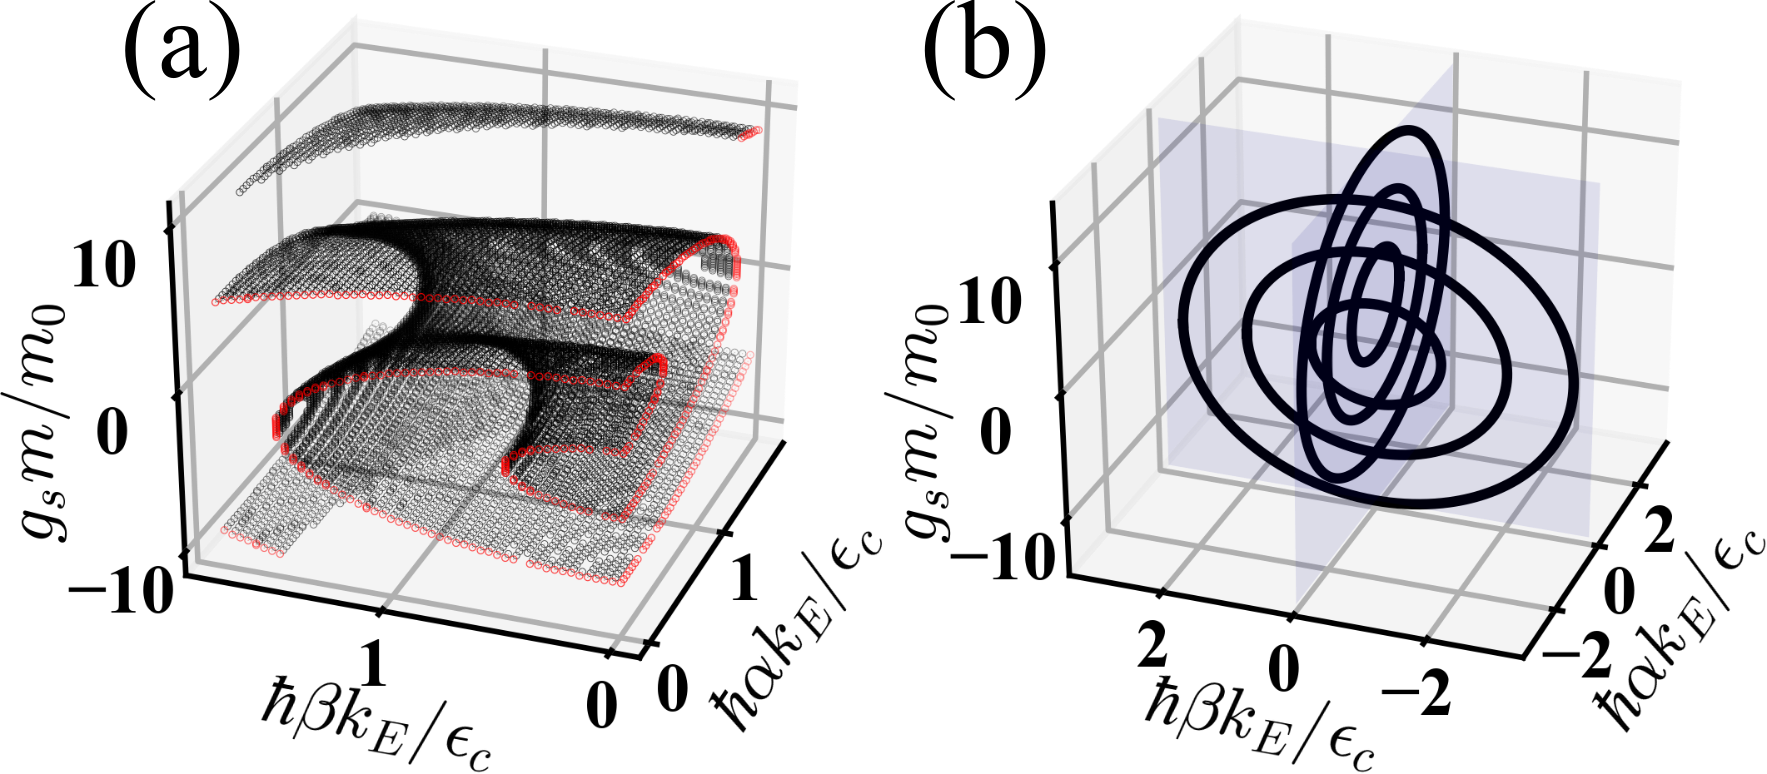
\includegraphics[width=1.0\columnwidth]{../figures/dgn.png}
	\centering
	\caption{Rashba-Dressalhaus模型的简并流形。 (a) $\A{=}I$的简并流形是一个道路连通的超曲面。 $\alpha=0$ 或者 $\beta=0$面上的点画成了红色。 (b) 阐释了$\A=-I$的简并流形,它处在$\alpha{=}0$和$\beta{=}0$面内(蓝色的半透明面)。这两个$\mathfrak{c}_{\infty}$对称的面都包含着无穷多的共心的圆。这两个面的圆相交在一起,因此整个流形是道路连通的 \label{fig:dgn}}
\end{figure}

\subsubsection{具有离散旋转对称性的Rashba-Dresselhaus二维电子气}\label{sec:disrot}

Rashba模型是一个过分的近似,连续旋转对称性不是任何晶体的对称性,连续旋转对称的$\bk{\cdot}\bp$模型仅仅是布洛赫哈密顿量的近似。那么如果连续旋转对称性微扰地降为离散的旋转对称性,上述的朗道能级的准简并会怎么变化呢?对于任意的整数$N{\geq}2$,我们发现$N$中的$N{-}1$个朗道能级准简并是稳定的,这一点的证明在附录\ref{app:codimension}。在这里,我们用一个$N{=}2$的模型来阐释上面的发现。我们要在Rashba模型中加入Dresselhaus自旋轨道耦合(耦合常数为$\beta$):
\begin{equation}
H_{RD}(\bk)=\frac{{\hbar^2}k^2}{2m}+\hbar\alpha(k_{x}\sigma_{y}-k_{y}\sigma_{x})+\hbar\beta(k_{x}\sigma_{x}-k_{y}\sigma_{y}).\label{hamRD}
\end{equation}
{For the Rashba-Dresselhaus 2DEG, $\A$ depends on $\alpha,~\beta,~l,~E,~m$ only through three independent parameters:}%$\hbar\alpha k_E /\var_c$, $\hbar\beta k_E /\var_c$ and $g_sm/m_0$, let us consider the three-dimensional parameter space:
\e{\left( \f{\hbar\alpha k_{\sma{E}}}{\var_c},\f{\hbar\beta k_{\sma{E}}}{\var_c},g_{s\perp}\f{m}{m_0} \right){\in} \mathbb{R}^3. \la{parameter2}}  
$\A(\hbar\alpha k_{\sma{E}}/\var_c,\hbar\beta k_{\sma{E}}/\var_c,g_{s\perp}m/m_0){=}{\pm} I$ then determines a set of concentric circles in the $\beta{=}0$ plane, as per the $\mathfrak{c}_{\infty}$-symmetric case study in \s{sec:ctsrot}. Moving off this plane, we find that $\A{=}I$ is satisfied in a  neighborhood of $\beta{=}0$, i.e., $\A{=}I$ defines a hypersurface in $\mathbb{R}^3$ that is illustrated in \fig{fig:dgn}(a). On the other hand, $\A{=}{-}I$ is not satisfied in the neighborhood of $\beta{=}0$, hence the circles associated to $\A{=}{-}I$ remain isolated as line nodes, as illustrated in \fig{fig:dgn}(b). To recapitulate, we have found that one of every two Landau-level crossings (those labelled by odd $j$) destabilize due to the symmetry reduction.

To demonstrate how the $\A{=}I$ hypersurface derives from $\mathfrak{c}_2$ symmetry, consider  the effective Hamiltonian $\calh$ 
\e{\calh=\hbar\alpha (k_{x}\sigma_{y}{-}k_{y}\sigma_{x})+\hbar\beta (k_{x}\sigma_{x}{-}k_{y}\sigma_{y})-\f{g_{s\perp}}{2}\mu_{B}B\sigma_z,}
in a momentum-independent basis where the Pauli matrices correspond to spin operators. The two-fold rotational symmetry 
\e{\calh(\bk)=\sigma_z\calh(-\bk)\sigma_z, \;\: \bk(t)=-\bk\big(t+\f{T_c}{2}\big)\in \frako_0,}
implies that the propagator over the time interval $[T_c/2,0]$ is symmetry-related to that over $[T_c,T_c/2]$:
\e{\A=\A_{T_c\leftarrow T_c/2}\A_{T_c/2\leftarrow 0}=\sigma_z{\A}_{T_c/2\leftarrow 0}\sigma_z {\A}_{T_c/2\leftarrow 0}.\label{eq:sigmazconstraint}}
The tracelessness of $\calh$ (at each $\bk$) implies that  ${\A}_{\sma{T_c/2\leftarrow 0}}$  has unit determinant. Employing the canonical SU(2) parametrization for the half-loop propagator [Eq. (\ref{s3}) with ${\cal \bar{A}}$ replaced by ${\A}_{\sma{T_c/2\leftarrow 0}}$], we derive from \q{eq:sigmazconstraint} that
\e{
	{\A}={\cal \bar{A}}(r_1,r_2,r_3)=\matrixtwo{1{-}2r_2(r_2{-}ir_1)}{2ir_2(r_3{+}ir_4)}{{-}2ir_2(r_3{-}ir_4)}{1{-}2r_2(r_2{+}ir_1)} \label{proprashba}
}
with $\sum_{j=1}^4r_j^2{=}1$. \q{proprashba} is a parametrization of the two-fold-symmetric propagator by the symmetric coordinates $\br{=}(r_1,r_2,r_3)$. It follows that $r_2{=}0$ is a necessary and sufficient condition for $\A{=}I$. The corresponding degeneracy manifold is a path-connected hypersurface, which separates $\br{=}(r_1,r_2,r_3)$-space into two distinct connected components. As proven in App. \ref{app:codimension}, this conclusion generalizes for any $N{\geq}2$: the degenerate manifolds of $\mathfrak{c}_N$-symmetric $\A$ separate the space of symmetric coordinates into $N$ distinct connected components. \fig{fig:dgn}(a) illustrates the $\A=I$ degenerate manifold {in the coordinates of  \q{parameter2} (which are distinct from the $\br$-coordinates in \q{proprashba}).} 

On the other hand, $\A{=}{-}I$ occurs if and only if $\br{=}(0,{\pm} 1,0)$. These two points are mapped to a path-connected line node confined to the $\alpha{=}0$ and $\beta{=}0$ planes [cf.\ \fig{fig:dgn}(b)]; the difference in codimension originates from the $\mathfrak{c}_{\infty}$ symmetry within these two planes (cf.\ \s{sec:ctsrot}), which was not accounted for in the $\mathfrak{c}_2$-symmetric analysis of \q{proprashba}.



